\documentclass[10pt]{article}
\usepackage[english]{babel}
\usepackage{../../../../lib/tex/naproche}
\usepackage{amssymb}
\usepackage{mathtools} % for \coloneq

\usepackage{stex-highlighting}
\providebool{emph} % "\newbool{emph}" does not work...
\setbool{emph}{false}
\colorlet{emphcolor}{violet}
\let\oldemph\emph
\renewcommand\emph[1]{\setbool{emph}{true}\ifbool{forthel}{\textcolor{emphcolor}{\itshape#1}}{\oldemph{#1}}\setbool{emph}{false}}
\renewcommand{\varemph}[1]{\ifbool{emph}{\textcolor{emphcolor}{#1}}{\textcolor{black}{#1}}}

\usepackage[right=6cm,left=3cm,bottom=3cm,marginparwidth=5cm]{geometry}

\usepackage{fancyhdr}
\renewcommand{\sectionmark}[1]{\markboth{#1}{}} 
\def\libarchive{}
\pagestyle{fancy}
\fancyhead[L]{\libarchive}
\fancyhead[C]{\nouppercase\leftmark}  % section title
\fancyhead[R]{\thepage}               % page number
\fancyfoot[C]{}                       % No page number in footer

\usepackage[nobottomtitles]{titlesec}
\titlespacing*{\section}{0pt}{30pt}{0pt}
\titlespacing*{\subsection}{0pt}{30pt}{0pt}
\titlespacing*{\subsubsection}{0pt}{30pt}{0pt}

\documentclass[12pt,oneside]{book}

\usepackage[foundations]{../../lib/tex/naproche}
\usepackage{../../lib/tex/libraries}
\usepackage{graphicx}
\usepackage{float}
\usepackage{caption}
\usepackage{footnote}

\makesavenoteenv{tabular} % Make footnotes work in tabular environments


\title{Foundations of Mathematics}
\author{Marcel Schütz}
\date{2022}

\begin{document}
  \maketitle

  \tableofcontents

  \begin{figure}[H]
    \centering
    \fbox{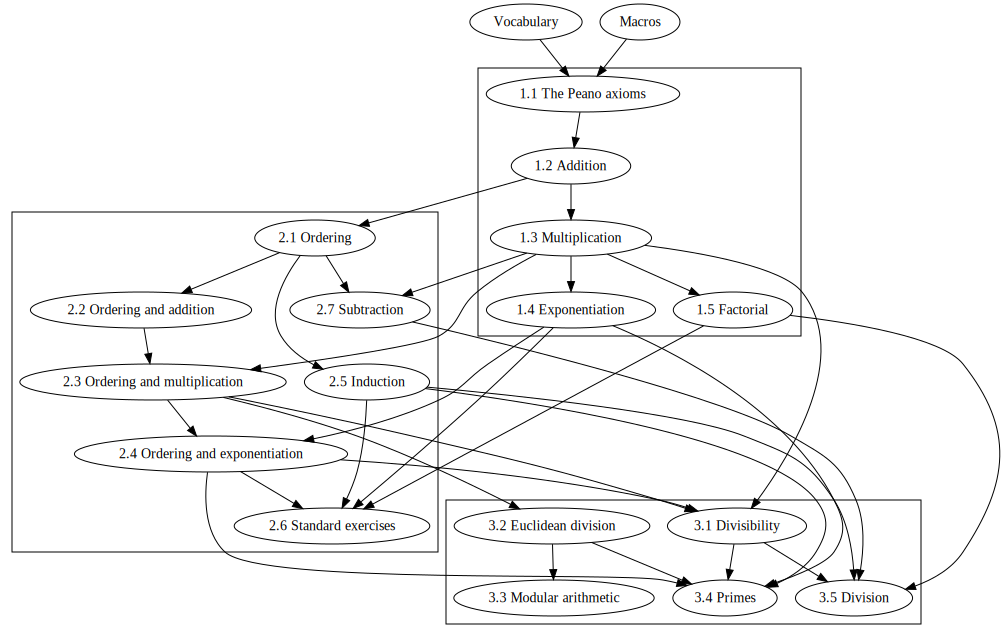
\includegraphics[width=0.9\linewidth]{./dependency-graph/graph.png}}
    \caption*{Interdependencies of the chapters}
  \end{figure}


  \section*{Introduction}

  This is a library providing a foundation of mathematics based on a
  Kelley-Morse like class theory with urelements.
  It introduces common operations on classes like unions or intersections
  (\cref{chapter:classes}) together with detailed proofs of their algebraic
  properties (\cref{chapter:computation-laws-for-classes}), the symmetric
  difference of two classes (\cref{chapter:symmetric-difference}) and the
  notions of ordered pairs and Cartesian products
  (\cref{chapter:pairs-and-products}) as well as proofs of the algebraic
  properties of the latter (\cref{chapter:computation-laws-for-products}).
  Moreover, it provides common operations on maps (\cref{chapter:maps}), various
  properties of images and preimages (\cref{chapter:image-and-preimage}) and the
  notions of injectivity, surjectivity, bijectivity
  (\cref{chapter:injections-surjections-bijections}) and invertibility of maps
  (\cref{chapter:invertible-maps}).
  The library provides an axiom system characterizing sets (\cref{chapter:sets})
  and, furthermore, it covers the notions of binary relations
  (\cref{chapter:binary-relations}), fixed-points of subset preserving maps
  (\cref{chapter:fixed-points}), including and equinumerosity
  (\cref{chapter:equinumerosity}).

  As two famous results it includes the Knaster-Tarski fixed point theorem
  (\cref{FOUNDATIONS_12_8420450166112256}) and the Cantor-Schröder-Bernstein
  theorem (\cref{FOUNDATIONS_13_1913663275401216}).

  \paragraph*{Usage.}
  At the very beginning of each chapter you can find the name of its source
  file, e.g. \path{foundations/sections/01_classes.ftl.tex} for
  \cref{chapter:classes}. This filename can be used to import the chapter via
  \Naproche's \texttt{readtex} instruction to another ForTheL text, e.g.:
  \begin{center}
    \verb`[readtex \path{foundations/sections/01_classes.ftl.tex}]`
  \end{center}

  \paragraph*{Checking times.}
  The checking times for each of the chapters may vary from computer to
  computer, but on mid-range hardware they are likely to be similar to those
  given in table below:

  \begin{center}
    \begin{tabular}{c|c|c}

      & \multicolumn{2}{c}{\textbf{Checking time}}
      \\
      \textbf{Chapter}
      & \textbf{without dependencies}     & \textbf{with dependencies}
      \\ \hline
      \ref{chapter:classes}
      & 00:04 min                         & 00:04 min
      \\
      \ref{chapter:computation-laws-for-classes}
      & 00:12 min                         & 00:16 min
      \\
      \ref{chapter:symmetric-difference}
      & 00:32 min                         & 00:48 min
      \\
      \ref{chapter:pairs-and-products}
      & 00:08 min                         & 00:12 min
      \\
      \ref{chapter:computation-laws-for-products}
      & 01:36 min                         & 01:56 min
      \\
      \ref{chapter:maps}
      & 01:13 min                         & 01:25 min
      \\
      \ref{chapter:image-and-preimage}
      & 01:28 min                         & 02:53 min
      \\
      \ref{chapter:injections-surjections-bijections}
      & 00:38 min                         & 02:03 min
      \\
      \ref{chapter:invertible-maps}
      & 02:20 min                         & 04:23 min
      \\
      \ref{chapter:sets}
      & 02:17 min                         & 06:40 min
      \\
      \ref{chapter:binary-relations}
      & 00:14 min                         & 06:54 min
      \\
      \ref{chapter:fixed-points}
      & 00:33 min                         & 07:13 min
      \\
      \ref{chapter:equinumerosity}
      & 01:48 min                         & 09:01 min
    \end{tabular}
  \end{center}


  \subfile{sections/01_classes.ftl.tex}
  \subfile{sections/02_computation-laws-for-classes.ftl.tex}
  \subfile{sections/03_symmetric-difference.ftl.tex}
  \subfile{sections/04_pairs-and-products.ftl.tex}
  \subfile{sections/05_computation-laws-for-products.ftl.tex}
  \subfile{sections/06_maps.ftl.tex}
  \subfile{sections/07_image-and-preimage.ftl.tex}
  \subfile{sections/08_injections-surjections-bijections.ftl.tex}
  \subfile{sections/09_invertible-maps.ftl.tex}
  \subfile{sections/10_sets.ftl.tex}
  \subfile{sections/11_binary-relations.ftl.tex}
  \subfile{sections/12_fixed-points.ftl.tex}
  \subfile{sections/13_equinumerosity.ftl.tex}
\end{document}

\usepackage{amssymb}

\newcommand{\Nat}{\mathbb{N}}
\newcommand{\Prime}{\mathbb{P}}
\renewcommand{\succ}{\textrm{succ}}
\newcommand{\pred}{\textrm{pred}}
\newcommand{\add}{\textrm{add}}
\newcommand{\mul}{\textrm{mul}}
\renewcommand{\exp}{\textrm{exp}}
\newcommand{\fac}{\textrm{fac}}
\renewcommand{\div}{\mathop{\textrm{div}}}
\renewcommand{\mod}{\mathop{\textrm{mod}}}

\begin{document}
  \begin{imports}
    \begin{forthel}
      %[prove off][check off]

      [readtex \path{libraries/source/arithmetics/02_recursion.ftl.tex}]

      %[prove on][check on]
    \end{forthel}
  \end{imports}


  \section{Definition of Addition}

  \begin{forthel}
    \begin{lemma}\printlabel{ARITHMETIC_03_722195546374144}
      There exists a $\varphi : \Nat \times \Nat \to \Nat$ such
      that for all $n \in \Nat$ we have $\varphi(n,0) = n$ and
      $\varphi(n,\succ(m)) = \succ(\varphi(n,m))$ for all $m \in \Nat$.
    \end{lemma}
    \begin{proof}
      Take $A = [\Nat \to \Nat]$.
      Define $a(n) = n$ for $n \in \Nat$.
      Then $A$ is a set and $a \in A$.

      [skipfail on] % Wrong proof task %!!
      Define $f(g) = \fun n \in \Nat. \succ(g(n))$ for $g \in A$.
      [skipfail off]

      Then $f : A \to A$.
      Indeed $f(g)$ is a map from $\Nat$ to $\Nat$ for any $g \in A$.
      Consider a $\psi : \Nat \to A$ such that $\psi$ is recursively defined by
      $a$ and $f$ (by \cref{ARITHMETIC_02_2489427471368192}).
      Define $\varphi(n,m) = \psi(m)(n)$ for $(n,m) \in \Nat \times \Nat$.
      Then $\varphi$ is a map from $\Nat \times \Nat$ to $\Nat$.

      (1) For all $n \in \Nat$ we have $\varphi(n,0) = n$. \\
      Proof.
        Let $n \in \Nat$.
        Then $\varphi(n,0)
          = \psi(0)(n)
          = a(n)
          = n$.
      Qed.

      (2) For all $n, m \in \Nat$ we have $\varphi(n, \succ(m)) =
      \succ(\varphi(n,m))$. \\
      Proof.
        Let $n, m \in \Nat$.
        Then $\varphi(n, \succ(m))
          = \psi(\succ(m))(n)
          = f(\psi(m))(n)
          = \succ(\psi(m)(n))
          = \succ(\varphi(n,m))$.
      Qed.
    \end{proof}
  \end{forthel}

  \begin{forthel}
    \begin{lemma}\printlabel{ARITHMETIC_04_2637025605844992}
      Let $\varphi, \varphi' : \Nat \times \Nat \to \Nat$.
      Assume that for all $n \in \Nat$ we have $\varphi(n,0) = n$ and
      $\varphi(n,\succ(m)) = \succ(\varphi(n,m))$ for all $m \in \Nat$.
      Assume that for all $n \in \Nat$ we have $\varphi'(n,0) = n$ and
      $\varphi'(n,\succ(m)) = \succ(\varphi'(n,m))$ for all $m \in \Nat$.
      Then $\varphi = \varphi'$.
    \end{lemma}
    \begin{proof}
      Define $\Phi = \{ m \in \Nat \mid \varphi(n,m) = \varphi'(n,m)$ for
      all $n \in \Nat \}$.

      (1) $0 \in \Phi$.
      Indeed $\varphi(n,0) = n = \varphi'(n,0)$ for all $n \in \Nat$.

      (2) For all $m \in \Phi$ we have $\succ(m) \in \Phi$. \\
      Proof.
        Let $m \in \Phi$.
        Then $\varphi(n,m) = \varphi'(n,m)$ for all $n \in \Nat$.
        Hence $\varphi(n, \succ(m))
          = \succ(\varphi(n,m))
          = \succ(\varphi'(n,m))
          = \varphi(n, \succ(m))$
        for all $n \in \Nat$.
      Qed.

      Thus $\Phi$ contains every natural number.
      Therefore $\varphi(n,m) = \varphi'(n,m)$ for all $n, m \in \Nat$.
    \end{proof}
  \end{forthel}

  \begin{forthel}
    \begin{definition}\printlabel{ARITHMETIC_03_4372222701469696}
      $\add$ is the map from $\Nat \times \Nat$ to $\Nat$ such that for all
      $n \in \Nat$ we have $\add(n,0) = n$ and $\add(n,\succ(m)) =
      \succ(\add(n,m))$ for all $m \in \Nat$.
    \end{definition}

    Let $n + m$ stand for $\add(n,m)$.
    Let the sum of $n$ and $m$ stand for $n + m$.
  \end{forthel}

  \begin{forthel}
    \begin{lemma}\printlabel{ARITHMETIC_03_3886414804549632}
      Let $n, m$ be natural numbers.
      Then $(n,m) \in \dom(\add)$.
    \end{lemma}
  \end{forthel}

  \begin{forthel}
    \begin{lemma}\printlabel{ARITHMETIC_03_5964925614686208}
      Let $n, m$ be natural numbers.
      Then $n + m$ is a natural number.
    \end{lemma}
  \end{forthel}

  \begin{forthel}
    \begin{lemma}\printlabel{ARITHMETIC_03_777009668030464}
      Let $n$ be a natural number.
      Then $\succ(n) = n + 1$.
    \end{lemma}
  \end{forthel}

  \begin{forthel}
    \begin{lemma}\printlabel{ARITHMETIC_03_4827955356237824}
      Let $n$ be a natural number.
      Then $n + 0 = n$.
    \end{lemma}
  \end{forthel}

  \begin{forthel}
    \begin{lemma}\printlabel{ARITHMETIC_03_1031280145727488}
      Let $n, m$ be natural numbers.
      Then $n + (m + 1) = (n + m) + 1$.
    \end{lemma}
  \end{forthel}


  \section{The Peano Axioms and Recursion, Revisited}

  \begin{forthel}
    \begin{proposition}\printlabel{ARITHMETIC_03_3170769680990208}
      Let $n, m$ be natural numbers.
      If $n + 1 = m + 1$ then $n = m$.
    \end{proposition}
  \end{forthel}

  \begin{forthel}
    \begin{proposition}\printlabel{ARITHMETIC_03_1101538491629568}
      Let $n$ be a natural number.
      Then $n + 1 \neq 0$.
    \end{proposition}
  \end{forthel}

  \begin{forthel}
    \begin{proposition}[Induction]\printlabel{ARITHMETIC_03_647949900054528}
      Let $A$ be a class.
      Assume $0 \in A$.
      Assume that for all $n \in \Nat$ if $n \in A$ then $n + 1 \in A$.
      Then $A$ contains every natural number.
    \end{proposition}
  \end{forthel}

  \begin{forthel}
    \begin{proposition}
      Let $a$ be an object and $f$ be a map.
      Let $\varphi$ be a map from $\Nat$ to $\dom(f)$.
      $\varphi$ is recursively defined by $a$ and $f$ iff $\varphi(0) = a$ and
      $\varphi(n + 1) = f(\varphi(n))$ for every $n \in \Nat$.
    \end{proposition}
  \end{forthel}


  \section{Computation Laws}

  \subsection{Associativity}

  \begin{forthel}
    \begin{proposition}\printlabel{ARITHMETIC_03_3235893452210176}
      Let $n, m, k$ be natural numbers.
      Then \[ n + (m + k) = (n + m) + k. \]
    \end{proposition}
    \begin{proof}
      Define $\Phi = \{ k' \in \Nat \mid n + (m + k') = (n + m) + k' \}$.

      (1) $0$ is contained in $\Phi$.
      Indeed $n + (m + 0) = n + m = (n + m) + 0$.

      (2) For all $k' \in \Phi$ we have $k' + 1 \in \Phi$. \\
      Proof.
        Let $k' \in \Phi$.
        Then $n + (m + k') = (n + m) + k'$.
        Hence
        \[  n + (m + (k' + 1))        \]
        \[    = n + ((m + k') + 1)    \]
        \[    = (n + (m + k')) + 1    \]
        \[    = ((n + m) + k') + 1    \]
        \[    = (n + m) + (k' + 1).   \]
        Thus $k' + 1 \in \Phi$.
      Qed.

      Thus every natural number is an element of $\Phi$.
      Therefore $n + (m + k) = (n + m) + k$.
    \end{proof}
  \end{forthel}


  \subsection{Commutativity}

  \begin{forthel}
    \begin{proposition}\printlabel{ARITHMETIC_03_4029553232052224}
      Let $n, m$ be natural numbers.
      Then \[ n + m = m + n. \]
    \end{proposition}
    \begin{proof}
      Define $\Phi = \{ m' \in \Nat \mid n + m' = m' + n \}$.

      (1) $0$ is an element of $\Phi$. \\
      Proof.
        Define $\Psi = \{ n' \in \Nat \mid n' + 0 = 0 + n' \}$.

        (1a) $0$ belongs to $\Psi$.

        (1b) For all $n' \in \Psi$ we have $n' + 1 \in \Psi$. \\
        Proof.
          Let $n' \in \Psi$.
          Then $n' + 0 = 0 + n'$.
          Hence
          \[  (n' + 1) + 0        \]
          \[    = n' + 1          \]
          \[    = (n' + 0) + 1    \]
          \[    = (0 + n') + 1    \]
          \[    = 0 + (n' + 1).   \]
        Qed.

        Hence every natural number belongs to $\Psi$.
        Thus $n + 0 = 0 + n$.
        Therefore $0$ is an element of $\Phi$.
      Qed.

      Let us show that (2) $n + 1 = 1 + n$. \\
      Proof.
        Define $\Theta = \{ n' \in \Nat \mid n' + 1 = 1 + n' \}$.

        (2a) $0$ is an element of $\Theta$.

        (2b) For all $n' \in \Theta$ we have $n' + 1 \in \Theta$. \\
        Proof.
          Let $n' \in \Theta$.
          Then $n' + 1 = 1 + n'$.
          Hence
          \[  (n' + 1) + 1        \]
          \[    = (1 + n') + 1    \]
          \[    = 1 + (n' + 1).   \]
          Thus $n' + 1 \in \Theta$.
        Qed.

        Thus every natural number belongs to $\Theta$.
        Therefore $n + 1 = 1 + n$.
      Qed.

      (3) For all $m' \in \Phi$ we have $m' + 1 \in \Phi$. \\
      Proof.
        Let $m' \in \Phi$.
        Then $n + m' = m' + n$.
        Hence
        \[  n + (m'  + 1)       \]
        \[    = (n + m') + 1    \]
        \[    = (m' + n) + 1    \]
        \[    = m' + (n + 1)    \]
        \[    = m' + (1 + n)    \]
        \[    = (m' + 1) + n.   \]
        Thus $m' + 1 \in \Phi$.
      Qed.

      Thus every natural number is an element of $\Phi$.
      Therefore $n + m = m + n$.
    \end{proof}
  \end{forthel}


  \subsection{Cancellation}

  \begin{forthel}
    \begin{proposition}\printlabel{ARITHMETIC_03_3137702874578944}
      Let $n, m, k$ be natural numbers.
      Then \[ n + k = m + k \implies n = m. \]
    \end{proposition}
    \begin{proof}
      Define $\Phi = \{ k' \in \Nat \mid$ if $n + k' = m + k'$ then $n = m \}$.

      (1) $0$ is an element of $\Phi$.

      (2) For all $k' \in \Phi$ we have $k' + 1 \in \Phi$. \\
      Proof.
        Let $k' \in \Phi$.
        Suppose $n + (k' + 1) = m + (k' + 1)$.
        Then $(n + k') + 1 = (m + k') + 1$.
        Hence $n + k' = m + k'$.
        Thus $n = m$.
      Qed.

      Therefore every natural number is an element of $\Phi$.
      Consequently if $n + k = m + k$ then $n = m$.
    \end{proof}
  \end{forthel}

  \begin{forthel}
    \begin{corollary}\printlabel{ARITHMETIC_03_8445946379632640}
      Let $n, m, k$ be natural numbers.
      Then \[ k + n = k + m \implies n = m. \]
    \end{corollary}
    \begin{proof}
      Assume $k + n = k + m$.
      We have $k + n = n + k$ and $k + m = m + k$.
      Hence $n + k = m + k$.
      Thus $n = m$.
    \end{proof}
  \end{forthel}


  \subsection{Zero Sums}

  \begin{forthel}
    \begin{proposition}\printlabel{ARITHMETIC_03_3520602170195968}
      Let $n, m$ be natural numbers.
      If $n + m = 0$ then $n = 0$ and $m = 0$.
    \end{proposition}
    \begin{proof}
      Assume $n + m = 0$.
      Suppose $n \neq 0$ or $m \neq 0$.
      Then we can take a $k \in \Nat$ such that $n = k + 1$ or $m = k + 1$.
      Hence there exists a natural number $l$ such that
      $n + m
        = l + (k + 1)
        = (l + k) + 1
        \neq 0$.
      Contradiction.
    \end{proof}
  \end{forthel}
\end{document}
